\documentclass[12pt, oneside]{article} 
\usepackage{amsmath, amsthm, amssymb, calrsfs, wasysym, verbatim, bbm, color, graphics, geometry, multirow, booktabs}
\usepackage{graphicx}
\usepackage{tikz}
\usepackage{amsmath}
\usepackage{graphicx}
\usepackage{amsmath, amssymb, amsthm}
\usepackage{setspace}
\usepackage{tikz}
\usetikzlibrary{trees, positioning}
\usepackage{pgfplots}
\renewcommand{\baselinestretch}{1.0}
\geometry{tmargin=.75in, bmargin=.75in, lmargin=.75in, rmargin = .75in}  

\newcommand{\R}{\mathbb{R}}
\newcommand{\C}{\mathbb{C}}
\newcommand{\Z}{\mathbb{Z}}
\newcommand{\N}{\mathbb{N}}
\newcommand{\Q}{\mathbb{Q}}
\newcommand{\Cdot}{\boldsymbol{\cdot}}


\newtheorem{thm}{Theorem}
\newtheorem{defn}{Definition}
\newtheorem{conv}{Convention}
\newtheorem{rem}{Remark}
\newtheorem{lem}{Lemma}
\newtheorem{cor}{Corollary}


\title{Game Theory}
\author{Kirby CHEN}
\date{Academic Year 2024-2025}

\begin{document}

\maketitle
\tableofcontents

\vspace{.25in}

\section{Nash Equilibrium in Pure Actions}

A game is triple (I,(A$_i$), (u$_i$)) where:
\begin{itemize}
    \item I is a set of players
    \item A$_i$ is the set of actions available to player i
    \item u$_i$ is the payoff function for player i
\end{itemize}

For the moment, the functions \( u_i \) represent ordinal preferences over \( \prod_{i \in I} A_i \).

Note that we are allowing arbitrary externalities.

Consider a game with \( N \) players. A strategy profile  
\[
\mathbf{s^*} = (s_1^*, s_2^*, \dots, s_N^*)
\]  
is a \textbf{Nash equilibrium} of the game if, for every player \( i \),

\[
u_i(s_i^*, \mathbf{s}_{-i}^*) \geq u_i(s_i', \mathbf{s}_{-i}^*)
\]

Given a game \( (I, (A_i)_{i \in I}, (u_i)_{i \in I}) \), a \underline{Nash equilibrium} of this game is an \( n \)-tuple of actions \( (a^*_i)_{i \in I} \) such that for every player \( i \in I \) and for every action \( a_i \in A_i \):

\[
u_i(a^*) \geq u_i(a_i, a^*_{-i}),
\]

where \( (a_i, a^*_{-i}) \) is the list of actions that is identical to \( a^* \) except that we have replaced \( a^*_i \) by \( a_i \).

\underline{\textbf{Interpretation:}} A Nash equilibrium represents a rest point of a learning process in which each player chooses the optimal action assuming that all other players choose the same actions as in the previous period.

\underline{\textbf{Best Response}}: A strategy \( s_i \) is a best response to a strategy profile \( s_{-i} \) if it maximizes the payoff of player i given the strategies of the other players.
\[
u_i(s_i, \mathbf{s}_{-i}) \geq u_i(s_i', \mathbf{s}_{-i})
\]

\underline{\textbf{Best Response Correspondence}}: The best response correspondence of player i is the correspondence that assigns to each strategy profile \( s_{-i} \) the set of best responses of player i to \( s_{-i} \).

\subsection{Key points}
\underline{\textbf{1. Nash equilibria are fixed points of the best reply correspondence.}}

For every player \( i \in I \) define a \underline{best reply correspondence} \( BR_i : \prod_{i \in I} A_i \rightrightarrows A_i \) by setting for every \( a \in \prod_{i \in I} A_i \):

\[
BR_i(a) = \{ a_i \in A_i \mid u_i(a_i, a_{-i}) \geq u_i(a'_i, a_{-i}) \text{ for every } a'_i \in A_i \}.
\]

The \underline{best reply correspondence} \( BR : \prod_{i \in I} A_i \rightrightarrows \prod_{i \in I} A_i \) is defined by setting for every \( a \in \prod_{i \in I} A_i \):

\[
BR(a) = \prod_{i \in I} BR_i(a).
\]

By definition: \( a^* \) is a Nash equilibrium if and only if \( a^* \in BR(a^*) \), i.e., if and only if \( a^* \) is a fixed point of \( BR \).



    \section{Static Games}

\subsection{Case 1: Betrend Competition}
In betrend competition, firm face a total cost curve for producing their goods and simply choose the price for their respective goods. 
Whichever firm has the lower price will get all the customers and if the prices are the same, the customers will be split evenly.
We will assume that identical firms face a constant marginal cost c. The firms simultaneously choose their prices, p1 and p2.
let's look at it from firm 1's perspective (it will be the same for firm firm 2). 

\textbf{Firm 1 has three strategies:}

\begin{itemize}
    \item $p_1 < p_2$: Firm 1 gets all the customers and makes a profit of $p_1 - c$.
    \item $p_1 = p_2$: Firm 1 gets half the customers and makes a profit of $\frac{p_1 - c}{2}$.
    \item $p_1 > p_2$: Firm 1 gets no customers and makes a profit of 0.
\end{itemize}

Naturally, depending on what firm 2's price is, we could have any of these situations. Let s look at some different conditions.

\begin{itemize}
    \item Starting with one extreme, suppose $p_2 > p^m$, the monopoly price.
    \begin{itemize}
        \item If firm 1 chose a price above this, firm 2 would get all of the consumers since their price is lower.
        \item If firm 1 matched this price, they would get half of the consumers.
        \item If firm 1 set a price lower than this, they would get all of the consumers.
    \end{itemize}
    \item Naturally, firm 1 would actually want to set $p_1 = p^m$ in this case since that’s the price that maximizes their profit level.
\end{itemize}

\begin{itemize}
    \item Now, let’s suppose firm 2 chose some price that was at most the monopoly price, i.e., $p_2 \leq p^m$. The same results hold.
    \begin{itemize}
        \item If firm 1 chose a price above this, firm 2 would get all of the consumers since their price is lower.
        \item If firm 1 matched this price, they would get half of the consumers.
        \item If firm 1 set a price lower than this, they would get all of the consumers.
    \end{itemize}
    \item It should be obvious that firm 1 wants to set a price lower than firm 2, $p_1 < p_2$. In fact, to maximize profit, firm 1 wants to undercut firm 2 by as little as possible (a single penny). $p_1 = p_2 - \varepsilon$ where $\varepsilon > 0$ is the smallest possible number that firm 1 can pick.
    \begin{itemize}
        \item That way they get all of the customers while lowering their profit margin by as little as possible.
    \end{itemize}
\end{itemize}

\begin{itemize}
    \item Lastly, suppose firm 2's price were at or below marginal cost, $p_2 \leq c$.
    \begin{itemize}
        \item If firm 1 chose a price above this, firm 2 would get all of the consumers since their price is lower.
        \item If firm 1 matched this price, they would get half of the consumers.
        \item If firm 1 set a price lower than this, they would get all of the consumers.
    \end{itemize}
    \item Pricing below marginal cost would not be an optimal strategy for firm 1. If $p_1 < c$, firm 1 would actually lose money on each unit sold.
    \begin{itemize}
        \item Thus, the lowest (and only possible) price firm 1 is willing to charge is $p_1 = c$.
    \end{itemize}
\end{itemize}

\begin{itemize}
    \item The analysis for firm 2 is identical.
    \begin{itemize}
        \item If firm 1 prices above the monopoly price, $p_2 = p^m$.
        \item If firm 1 prices between marginal cost and the monopoly price, $p_2 = p_1 - \varepsilon$, where $\varepsilon > 0$ is the smallest possible number greater than zero.
        \item If firm 1 prices at or below marginal cost, $p_2 = c$.
    \end{itemize}
\end{itemize}

\begin{itemize}
    \item Returning to our Nash equilibrium solution concept, we know that our equilibrium is when neither firm has any incentive to deviate from their chosen strategy.
    \begin{itemize}
        \item This occurs where the best response functions intersect.
    \end{itemize}
    \item There is exactly one intersection point in the previous figure, where $p_1 = p_2 = c$. Thus, both firms price at marginal cost in equilibrium.
    \begin{itemize}
        \item This should make sense. Each firm wants to undercut the other to claim the whole market. Yet they can’t undercut anymore once the price is at marginal cost or they’ll suffer losses.
        \item Bertrand competition implies that with just two firms, we reach the perfectly competitive equilibrium.
    \end{itemize}
    \item Since price is set at marginal cost for both firms, economic profit under Bertrand competition equals zero.
\end{itemize}

\begin{figure}[h!]
    \centering
    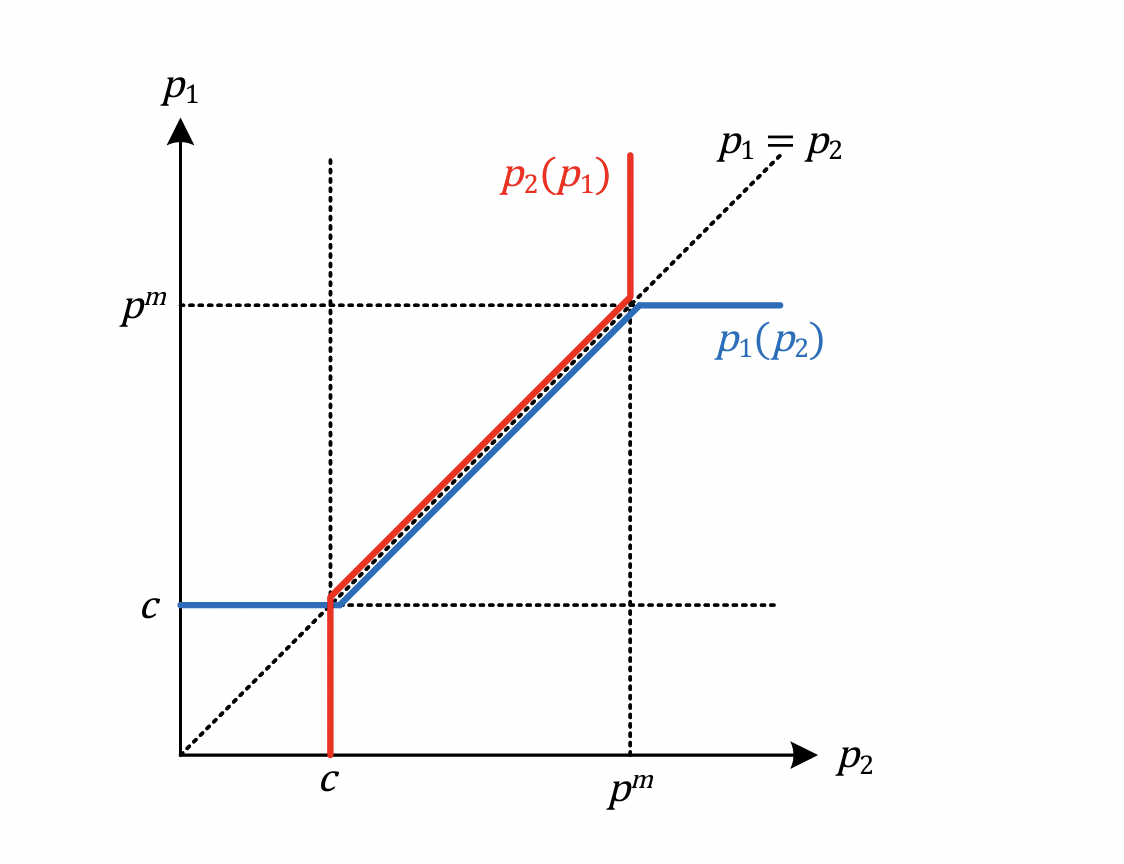
\includegraphics[width=0.8\textwidth]{Figure/Betrend.png}
    \caption{EQ} 
    \label{fig:1} 
\end{figure}
\break
\subsection{Case 2: Cournet Competition}

Now back to the last example in the previous lecture. Suppose the market has two oligopolists. The market
has the same inverse demand function as before: with \( a, b > 0 \),

\[
p(q) =
\begin{cases}
a - bq & \text{if } q < \frac{a}{b} \\
0 & \text{if } q \geq \frac{a}{b}
\end{cases}
\]

Here, \( q = q_1 + q_2 \), where \( q_1 \) and \( q_2 \) are the quantities chosen by the oligopolists respectively. They choose their quantity without knowing their opponent’s choice. They produce goods with the same constant marginal cost \( c \in [0,a] \). And both of them maximize their profit, i.e., the first monopolist solves:

\[
\max_{q_1 \geq 0} p(q_1 + q_2) q_1 - c q_1
\]

and the second monopolist solves:

\[
\max_{q_2 \geq 0} p(q_1 + q_2) q_2 - c q_2
\]

To find the Nash equilibrium, let’s first solve for the best response of each firm. Firm 1’s best response can be obtained by solving

\[
\max_{q_1 \geq 0} p(q_1 + q_2) q_1 - c q_1
\]

If \( q_2 \geq \frac{a}{b} \), then \( p(q) = 0 \). In this case, it is optimal for Firm 1 to choose \( q_1 = 0 \).

Now consider \( q_2 < \frac{a}{b} \). If Firm 1 chooses \( q_1 \geq \frac{a}{b} - q_2 \), then firm 1’s payoff is negative. Now consider firm 1 chooses \( q_1 \in [0, \frac{a}{b} - q_2] \). Firm 1 solves the following problem.

\[
\max_{q_1 \in [0, \frac{a}{b} - q_2]} (a - b q_1 - b q_2) q_1 - c q_1
\]

The first order derivative with respect to \( q_1 \) is given by

\[
a - c - b q_2 - 2 b q_1
\]

This is positive when \( q_1 < \frac{a - c - bq_2}{2b} \) and is negative when \( q_1 > \frac{a - c - bq_2}{2b} \). If \( \frac{a - c - bq_2}{2b} \leq 0 \), it is optimal for Player 1 to choose \( q_1 = 0 \). If \( \frac{a - c - bq_2}{2b} > 0 \), it is optimal for Player 1 to choose \( \frac{a - c - bq_2}{2b} \), which yields a positive payoff.

Summarizing the above, Player 1’s best response is given by the following:

\[
b_1(q_2) =
\begin{cases}
    \{0\} & \text{if } q_2 \geq \frac{a - c}{b} \\
    \left\{ \frac{a - c - bq_2}{2b} \right\} & \text{if } q_2 < \frac{a - c}{b}
\end{cases}
\]

Symmetrically, Player 2’s best response is given by the following:

\[
b_2(q_1) =
\begin{cases}
    \{0\} & \text{if } q_1 \geq \frac{a - c}{b} \\
    \left\{ \frac{a - c - bq_1}{2b} \right\} & \text{if } q_1 < \frac{a - c}{b}
\end{cases}
\]

We similarly use figures to find the Nash equilibrium.
\begin{center}
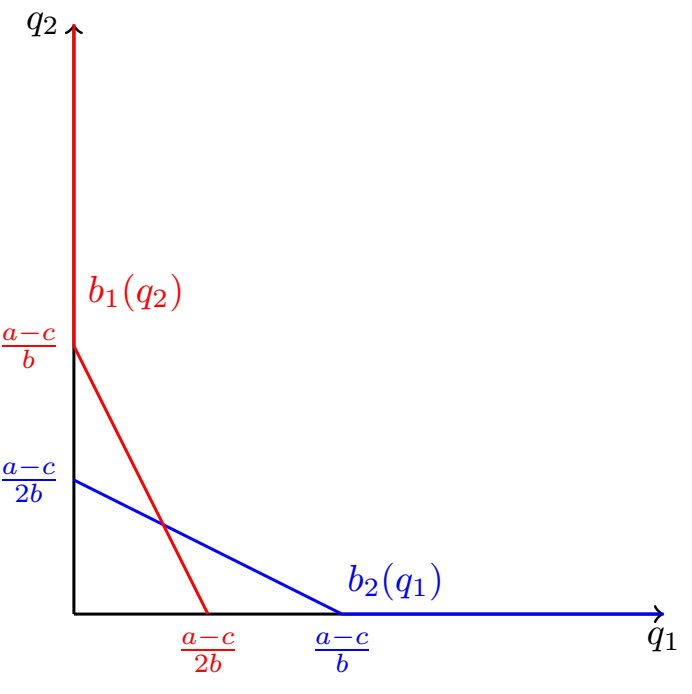
\includegraphics{Figure/Cournet.jpg}
\end{center}
The best response correspondences cross once where

\[
q_1 = \frac{a - c - bq_2}{2b}
\]

\[
q_2 = \frac{a - c - bq_1}{2b}
\]

Solving the above equations, we have

\[
q_1 = q_2 = \frac{a - c}{3b}
\]

The total market output is

\[
q = q_1 + q_2 = \frac{2(a - c)}{3b}
\]

The equilibrium price is

\[
p(q) = \frac{a + 2c}{3}
\]

\subsection{Trembling Hand Perfection}

\textbf{Definition 13.} A Nash equilibrium $\sigma$ of game $\Gamma_N = [I, \{\Delta(S_i)\}, \{u_i(\cdot)\}]$ is a trembling-hand perfect if and only if there is some sequence of totally mixed strategies $\{\sigma^k\}_{k=1}^{\infty}$ such that $\lim_{k \to \infty} \sigma^k = \sigma$ and $\sigma_i$ is a best response to every element of sequence $\{\sigma_{-i}^k\}_{k=1}^{\infty}$ for all $i = 1,2, \dots, I$.

Totally mixed strategy means a strategy that assigns positive probabilities to each action. We will see a similar idea in lecture 6.

\textbf{Example}
Let's find all pure-strategy trembling-hand perfect Nash equilibrium of the following game.

\begin{center}
\begin{tabular}{c|cc}
 & \textbf{Player 2} & \\
\textbf{Player 1} & L & R \\
\hline
U & 1,1 & 0,-3 \\
D & -3,0 & 0,0 \\
\end{tabular}
\end{center}

There are two pure-strategy Nash equilibria: (U,L) and (D,R).

First, we show that (D,R) is not trembling-hand perfect. Consider $\{\sigma^k\}_{k=1}^{\infty}$ such that player 1 chooses U with probability $p^k \in (0,1)$ and chooses D with probability $1 - p^k$, and player 2 choose L with probability $q^k$ and choose R with probability $1 - q^k$, where $q^k \in (0,1)$. Then payoff of player 1 from action U is $q^k > 0$. The payoff of player 1 from action D is $-3q^k < 0$. Therefore, D is not a best response to any totally mixed strategy of player 2, making (D,R) not a trembling-hand perfect Nash equilibrium.

Next, we show that (U,L) is trembling-hand perfect. Based on the discussion above, U is a best response to any totally mixed strategies of player 2. One can similarly see that L is a best response to any totally mixed strategies of player 1, making (U,L) a trembling-hand perfect Nash equilibrium.

Notice that we just need the equilibrium strategy to be a best response to a sequence, not all possible sequences. That means, as long as for some form of mistakes, the equilibrium strategy is the best, the equilibrium is trembling hand perfect.

In the example, D and R are weakly dominated strategies. (D,R) is not trembling-hand perfect. This is not a coincidence. We have the following more general result.

\textbf{Definition 14.} If $\sigma = (\sigma_1, \sigma_2, \dots, \sigma_n)$ is a trembling-hand perfect Nash equilibrium, then $\sigma_i$ is not a weakly dominated strategy for any $i = 1,2, \dots, n$.

\textbf{Example: MWG, page 265: Exercise 8.F. 2}
Consider the following three-player game [taken from van Damme (1983)], in which player 1 chooses rows ($S_1 = \{U,D\}$), player 2 chooses columns ($S_2 = \{L,R\}$), and player 3 chooses boxes ($S_3 = \{B_1,B_2\}$):

\begin{center}
\textbf{B$_1$}
\[
\begin{array}{c|cc}
    & L & R  \\
\hline
U & 1,1,1 & 1,0,1 \\
D & 1,1,1 & 0,0,1 \\
\end{array}
\]
\hspace{1cm}
\textbf{B$_2$}
\[
\begin{array}{c|cc}
    & L & R  \\
\hline
U & 1,1,0 & 0,0,0 \\
D & 0,1,0 & 1,0,0 \\
\end{array}
\]
\end{center}

Each cell describes the payoffs to the three players ($u_1, u_2, u_3$) from that strategy combination. Both $(D,L,B_1)$ and $(U,L,B_1)$ are pure strategy Nash equilibria. Show that $(D,L,B_1)$ is not (normal form) trembling-hand perfect even though none of these three strategies is weakly dominated.

\textbf{Solution:}

We define $\delta^t = ((\varepsilon_1, 1 - \varepsilon_1), (1 - \varepsilon_2, \varepsilon_2), (1 - \varepsilon_3, \varepsilon_3))$ which converges to $\delta = (\delta_1, \delta_2, \delta_3) = ((0,1), (1,0), (1,0)) = (D, L, B_1)$ as $t \to \infty$. ($\varepsilon_i \to 0$ as $t \to \infty$ for all $i$.) To show that $(D,L,B_1)$ is not (normal form) trembling-hand perfect, we should have, for some $i$ and $t$,

\begin{equation}
\pi_i(\delta_i, \delta^t_{-i}) < \pi_i(s_i, \delta^t_{-i}) \quad \text{for some } s_i \in S_i.
\end{equation}

We are going to compare $\pi_1(\delta_1, \delta^t_{-1}) = \pi_1(D, (1 - \varepsilon_2, \varepsilon_2), (1 - \varepsilon_3, \varepsilon_3))$ and $\pi_1(s_1, \delta^t_{-1}) = \pi_1(U, (1 - \varepsilon_2, \varepsilon_2), (1 - \varepsilon_3, \varepsilon_3))$.

\begin{equation}
\pi_1(D, (1 - \varepsilon_2, \varepsilon_2), (1 - \varepsilon_3, \varepsilon_3))
\end{equation}
\[
= (1 - \varepsilon_2)(1 - \varepsilon_3) \times 1 + (1 - \varepsilon_2)\varepsilon_3 \times 0 + \varepsilon_2(1 - \varepsilon_3) \times 0 + \varepsilon_2\varepsilon_3 \times 1
\]
\[
= 1 - \varepsilon_2 - \varepsilon_3 + 2\varepsilon_2\varepsilon_3.
\]

\begin{equation}
\pi_1(U, (1 - \varepsilon_2, \varepsilon_2), (1 - \varepsilon_3, \varepsilon_3))
\end{equation}
\[
= (1 - \varepsilon_2)(1 - \varepsilon_3) \times 1 + (1 - \varepsilon_2)\varepsilon_3 \times 1 + \varepsilon_2(1 - \varepsilon_3) \times 1 + \varepsilon_2\varepsilon_3 \times 0
\]
\[
= 1 - \varepsilon_2\varepsilon_3.
\]

\begin{equation}
\pi_1(U, (1 - \varepsilon_2, \varepsilon_2), (1 - \varepsilon_3, \varepsilon_3)) - \pi_1(D, (1 - \varepsilon_2, \varepsilon_2), (1 - \varepsilon_3, \varepsilon_3))
\end{equation}
\[
= (1 - \varepsilon_2\varepsilon_3) - (1 - \varepsilon_2 - \varepsilon_3 + 2\varepsilon_2\varepsilon_3)
\]
\[
= \varepsilon_2 + \varepsilon_3 - \varepsilon_2\varepsilon_3 = \varepsilon_2\varepsilon_3 \left(\frac{1}{\varepsilon_3} + \frac{1}{\varepsilon_2} - 1\right).
\]

If $t$ is sufficiently high, or in other words if $\varepsilon_i$'s are sufficiently small, (6) is positive.
\[
\left(\frac{1}{\varepsilon_3} + \frac{1}{\varepsilon_2} - 1\right) > 0
\]

Hence,

\begin{equation}
\pi_1(\delta_1, \delta^t_{-1}) = \pi_1(D, (1 - \varepsilon_2, \varepsilon_2), (1 - \varepsilon_3, \varepsilon_3)) < \pi_1(s_1, \delta^t_{-1}) = \pi_1(U, (1 - \varepsilon_2, \varepsilon_2), (1 - \varepsilon_3, \varepsilon_3)).
\end{equation}

Therefore, we conclude that $(D, L, B_1)$ is not (normal form) trembling-hand perfect.

\section{Nash Equilibria in Mixed Actions}
\section{Commplete Information Dynamic Games}
\subsection{Entry Game}
A firm called Firm E is considering entering a market that currently has a single incumbent Firm I. If it chooses “in”, the incumbent can respond in one of the two ways: It can either accomodate the entrant, of fight the entrant. We use the following tree to represent the whole process.

\begin{tikzpicture}[
    scale=1, 
    every node/.style={scale=1},
    grow=right, 
    sibling distance=5cm, 
    level distance=3cm,
    edge from parent path={(\tikzparentnode.east) -- (\tikzchildnode.west)}
]

\node[circle,draw] {} 
    child { node {Firm E}
        child { node {Out} 
            child { node {$(0,2)$} edge from parent[draw=none]}
            edge from parent node[above] {Out} 
        }
        child { node[circle,fill,inner sep=2pt] {} 
            child { node {Fight}
                child { node {$(-3,-1)$} edge from parent[draw=none]}
                edge from parent node[above] {Fight} 
            }
            child { node {Accomodate}
                child { node {$(2,1)$} edge from parent[draw=none]}
                edge from parent node[above] {Accomodate} 
            }
            edge from parent node[above] {In} 
            node[right=2mm] {Firm I}
        }
    };

\end{tikzpicture}


\section{Incomplete Information}
A game has (is of) incomplete information when at least one player does not know the payoff that some player receives from some strategy profile (or terminal nodes).

In this section, we will consider simultaneously-move games with incomplete information.

As an example, consider the following game. This is a modified Prisoner’s dilemma. Prisoner 1 is not clear about the crime she committed so she doesn’t know which of the following games is played.

Prisoner 2, on the other, has more knowledge about law so he knows which game is played.

\begin{table}[h]
    \centering
    \renewcommand{\arraystretch}{1.2}
    \setlength{\tabcolsep}{8pt}
    \begin{tabular}{c c|c c|}
        \multicolumn{2}{c}{} & \multicolumn{2}{c}{\textbf{Prisoner 2}} \\
        \multicolumn{2}{c}{} & Defense & Confess \\
        \cline{2-4}
        \multirow{2}{*}{\textbf{Prisoner 1}} & Defense & -2,-2 & -10,-1 \\
        & Confess & -1,-10 & -5,-5 \\
        \cline{2-4}
        \multicolumn{4}{c}{Good}
    \end{tabular}
    \hspace{1cm}
    \begin{tabular}{c c|c c|}
        \multicolumn{2}{c}{} & \multicolumn{2}{c}{\textbf{Prisoner 2}} \\
        \multicolumn{2}{c}{} & Defense & Confess \\
        \cline{2-4}
        \multirow{2}{*}{\textbf{Prisoner 1}} & Defense & -5,-5 & -13,-4 \\
        & Confess & -4,-13 & -8,-8 \\
        \cline{2-4}
        \multicolumn{4}{c}{Bad}
    \end{tabular}
\end{table}
\break
Let's use a game tree to represent this. In the eyes of Prisoner 1, this game is like this:

\begin{center}
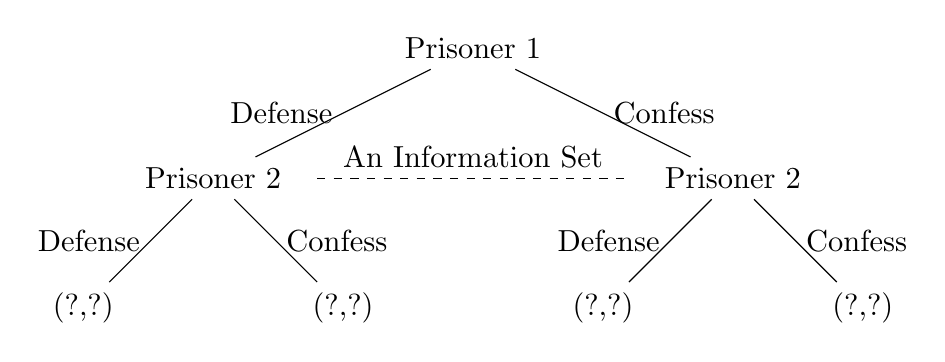
\begin{tikzpicture}[scale=1.1, transform shape]
    \tikzstyle{level 1}=[sibling distance=60mm]
    \tikzstyle{level 2}=[sibling distance=30mm]
    
    \node {Prisoner 1}
        child { node {Prisoner 2}
            child { node { (?,?) } edge from parent node[left] {Defense} }
            child { node { (?,?) } edge from parent node[right] {Confess} }
            edge from parent node[left] {Defense}
        }
        child { node {Prisoner 2}
            child { node { (?,?) } edge from parent node[left] {Defense} }
            child { node { (?,?) } edge from parent node[right] {Confess} }
            edge from parent node[right] {Confess}
        };
    
    % Drawing the information set
    \draw[dashed] (-1.8,-1.5) -- (1.8,-1.5) node[midway, above] {An Information Set};
\end{tikzpicture}
\end{center}

\subsection{Types and strategies}
Dealing with games with incomplete information is difficult. But Harsany came up with a solution to address this problem. His idea is to transform any game of incomplete information into a game with complete but imperfect information.

When doing so, we suppose the nature randomly chooses a “type” for each player. Each player knows only her own type, but not other players' type. The types of all players influence the payoff of each player.

For example, after introducing the nature and type, then we can say Prison 2 has 2 types: Good or Bad. Prisoner 2's type not only influences his own payoff, it also influences the payoff of Prisoner 1.
The game tree now looks like the following.
\begin{figure}[h!]
    \centering
    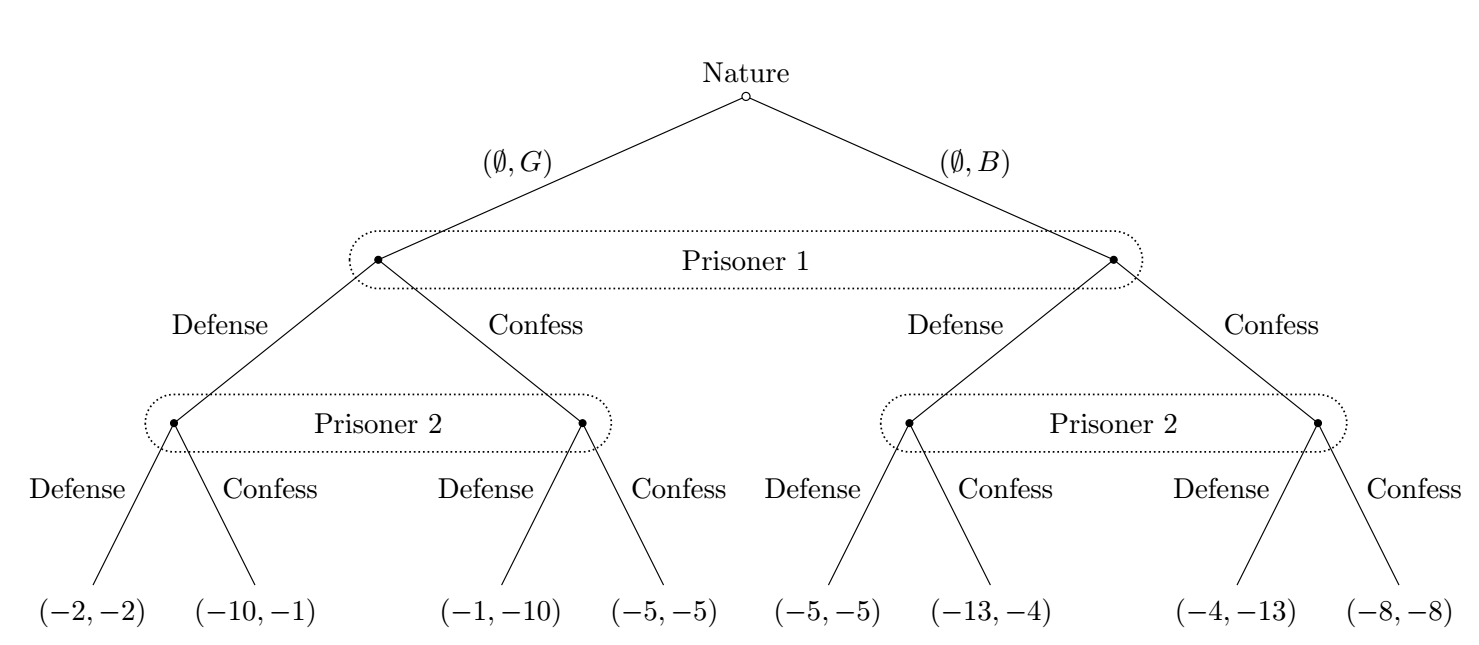
\includegraphics[width=0.8\textwidth]{Figure/incom_tree.png} 
    \caption{Incomplete Information Game Tree} 
    \label{fig:2} 
\end{figure}

\break
Prisoner 1 cannot distinguish the two decision nodes because she cannot observe the type of Prisoner 2.
Prisoner 2 has 2 types, and he can observe his own type, so he has 2 information sets.

We can still define a strategy as a function that maps an information set to a distribution over actions.
Now an information set just represents a type of a player. Here, Prisoner 1 has only one type, so she has only one information set.

Thus, we can also define a strategy as a function from a type to a distribution over action.

More formally, a static game of incomplete information can be described by:
\[
\Gamma_N = [I, \{\Delta(A_i)\}_{i \in I}, \{u_i(\cdot)\}_{i \in I}, \{\Theta_i\}_{i \in I}]
\]
such that:

\begin{enumerate}
    \item \( I \): a set of players. We assume there are \( n \) players.
    \item \( \Delta(A_i) \): the set of mixed action of player \( i \).
    \item \( \Theta_i \): a set of types of player \( i \). We define \( \Theta = \Theta_1 \times \Theta_2 \times \cdots \times \Theta_n \) and \( (\theta_i, \theta_{-i}) \) to define a type profile, where \( \theta_{-i} = (\theta_j)_{j \neq i} \).
    \item \( u_i : \prod_{j=1}^{n} \Delta(A_i) \times \prod_{j=1}^{n} \Theta_j \to \mathbb{R} \): the utility function of player \( i \), which depends on the action profile and players’ types. We use \( u_i(\alpha_1, \alpha_2, \dots, \alpha_n, \theta_1, \theta_2, \dots, \theta_n) \) to denote the expected payoff of player \( i \) when the action profile is \( (\alpha_1, \alpha_2, \dots, \alpha_n) \) and the type profile is \( (\theta_1, \theta_2, \dots, \theta_n) \).
\end{enumerate}

In the above example, \( I = \{1,2\} \), \( A_i = \{D,C\} \), \( \Theta_1 = \{\emptyset\} \) and \( \Theta_2 = \{G, B\} \). The utility function of P1 is such that \( u_1(D, D, \emptyset, G) = -2 \) and so on.

A pure strategy of player \( i \) is a function \( s_i : \Theta_i \to A_i \) such that \( s_i(\theta) \) is the action chosen by player \( i \) of type \( \theta \in \Theta_i \).

A mixed strategy of player \( i \) is a function \( \sigma_i : \Theta_i \to \Delta(A_i) \) such that \( \sigma_i(a | \theta) \) is the probability that action \( a \in A_i \) is chosen by player \( i \) of type \( \theta \in \Theta_i \). If \( A_i \) has \( m \) elements, we can also use \( \sigma_i(\theta) = (p_1, p_2, \dots, p_m) \) to represent a strategy of player \( i \) of type \( \theta \).

So for Player 1, \( s_1(\emptyset) = D \) is a pure strategy. For Player 2, \( \sigma_2(G) = \left( \frac{1}{2}, \frac{1}{2} \right) \) and \( \sigma_2(B) = (1,0) \) is a mixed strategy.

\subsection{Dominant and Dominated Strategies}
The idea of dominant and dominated strategies can be extended to an incomplete information game. We give the following definitions.

\textbf{Definition 1.} In an incomplete information game 
\[
\Gamma_N = [I, \{\Delta(A_i)\}_{i\in I}, \{u_i(\cdot)\}_{i\in I}, \{\Theta_i\}_{i\in I}],
\]
a strategy \(\sigma_i\) is said to strictly dominate \(\sigma'_i\) if for all \((\theta_i, \theta_{-i}) \in \Theta\) and all \(a_{-i} \in \prod_{j \neq i} A_j\),
\[
u_i(\sigma_i(\theta_i), a_{-i}, \theta_i, \theta_{-i}) > u_i(\sigma'_i(\theta_i), a_{-i}, \theta_i, \theta_{-i}).
\]
The strategy \(\sigma_i\) is strictly dominant if it strictly dominates every other strategy \(\alpha'_i\).

\vspace{0.5cm}

A strategy profile \((\sigma_1, \sigma_2, \dots, \sigma_n)\) is a strictly dominant strategy equilibrium if \(\sigma_i\) is a strictly dominant strategy for all \(i\).

In the previous example, regardless of the type of Player 2, for both players, Confess is a strictly dominant strategy so we can predict that both players of any type choose Confess.

The above condition is too strong. We also state a weaker one as below.

\vspace{0.5cm}

\textbf{Definition 2.} In an incomplete information game \[
\Gamma_N = [I, \{\Delta(A_i)\}_{i\in I}, \{u_i(\cdot)\}_{i\in I}, \{\Theta_i\}_{i\in I}],
\]
a strategy \(\sigma_i\) is said to weakly dominate \(\sigma'_i\) if for all \((\theta_1, \theta_2, \dots, \theta_n) \in \Theta\) and all \(a_{-i} \in \prod_{j \neq i} A_j\),
\[
u_i(\sigma_i(\theta_i), a_{-i}, \theta_i, \theta_{-i}) \geq u_i(\sigma'_i(\theta_i), a_{-i}, \theta_i, \theta_{-i})
\]
with strictly inequality for some \(a_{-i}\) and \((\theta_i, \theta_{-i})\).

The strategy \(\sigma_i\) is weakly dominant if it weakly dominates every other strategy \(\alpha'_i\).

A strategy profile \((\sigma_1, \sigma_2, \dots, \sigma_n)\) is a weakly dominant strategy equilibrium if \(\sigma_i\) is a weakly dominant strategy for all \(i\).

\subsection{Beliefs and Bayesian Games}
Now we change the payoff in the previous example a little bit. We still assume Player 1 does not know which game is played and thus is of one type, while Player 2 knows which game is played and has 2 types.

\begin{table}[h]
    \renewcommand{\arraystretch}{1.2}
    \setlength{\tabcolsep}{8pt}
    \begin{tabular}{c c|c c|}
        \multicolumn{2}{c}{} & \multicolumn{2}{c}{\textbf{Prisoner 2}} \\
        \multicolumn{2}{c}{} & Defense & Confess \\
        \cline{2-4}
        \multirow{2}{*}{\textbf{Prisoner 1}} & Defense & -2,-2 & -10,-1 \\
        & Confess & -1,-10 & -5,-5 \\
        \cline{2-4}
        \multicolumn{4}{c}{Good}
    \end{tabular}
    \hspace{1cm}
    \begin{tabular}{c c|c c|}
        \multicolumn{2}{c}{} & \multicolumn{2}{c}{\textbf{Prisoner 2}} \\
        \multicolumn{2}{c}{} & Defense & Confess \\
        \cline{2-4}
        \multirow{2}{*}{\textbf{Prisoner 1}} & Defense & -4,-5 & -8,-4 \\
        & Confess & -5,-13 & -13,-8 \\
        \cline{2-4}
        \multicolumn{4}{c}{Bad}
    \end{tabular}
\end{table}

Prisoner 1 has no dominant strategy now. If Prisoner 2's type is Good, it is optimal for Player 1 to choose Confess. If his type is Bad, it is optimal to choose Defense.

We want to have an incomplete information game version of Nash equilibrium, which we can guarantee its existence and it is an extension of the previous concepts. To do so, we will have to specify how Prisoner 1 thinks of Prisoner 2's type. Or how Prisoner 1 assigns probabilities to the two decision nodes in her information set. We introduce the following concept.

\textbf{Definition 3.} In an extensive form game \( \Gamma_E \), a belief system \( \mu : N \to [0,1] \) assigns probability to each decision node such that for any information set \( h \in H \),
\[
\sum_{x \in h} \mu(x) = 1
\]

In our example, we need to specify \( \mu(x_1) \) and \( \mu(x_2) \), the probabilities that Prisoner 1 assigns to the 2 decision nodes in her information set.

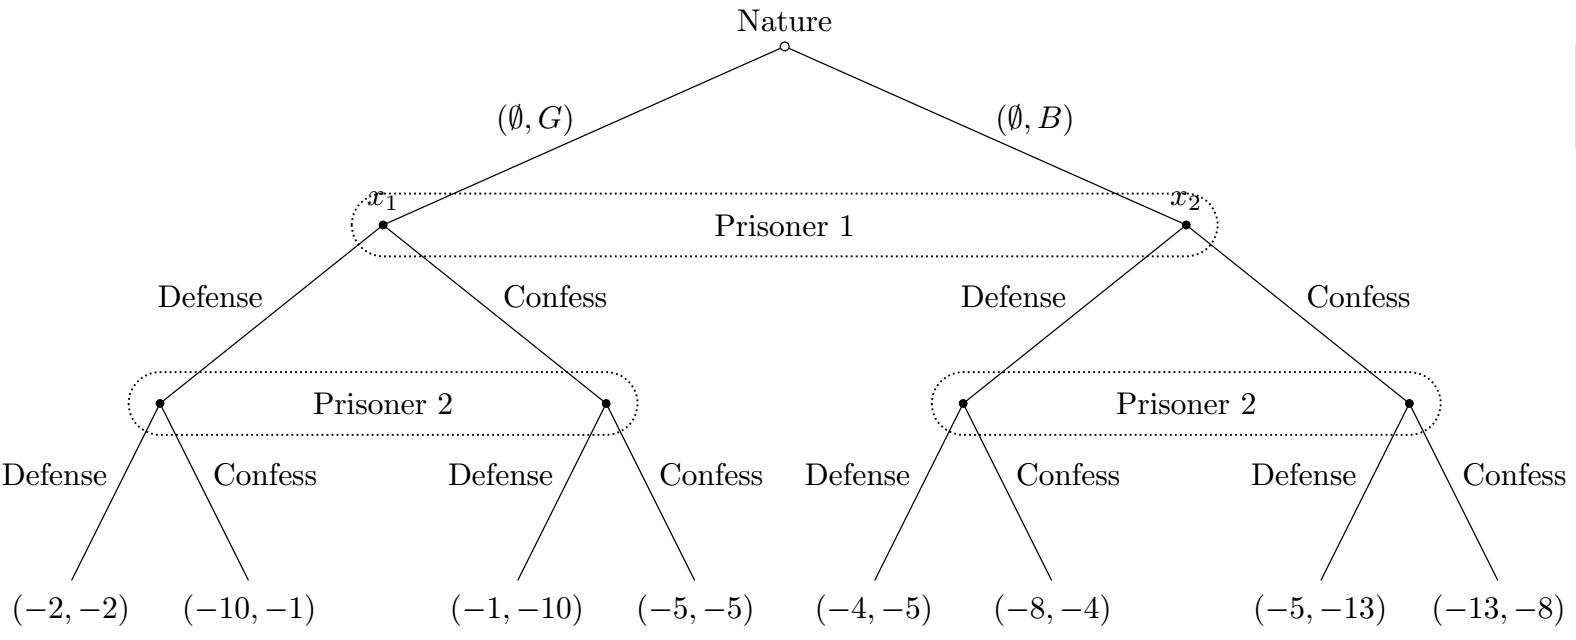
\includegraphics{Figure/incom_tree_bey.png}

To specify the beliefs of players, we usually assume the incomplete information games we consider are Bayesian games. In addition to what constitutes an incomplete information game, in a Bayesian game, nature assigns probabilities to type profiles of the players.

A Bayesian game is an incomplete information game with a probability distribution \( p \) over type profiles \( \Theta = \Theta_1 \times \Theta_2 \times \cdots \times \Theta_n \). We assume this distribution \( p \) is a common knowledge.

When each player has finite types, we use a probability mass function \( p \) such that \( p(\theta_1, \theta_2, \dots, \theta_n) \) is the probability the nature assigns to type profile \( (\theta_1, \theta_2, \dots, \theta_n) \). When types are real numbers, \( p \) is the probability density function.

We use 
\[
\Gamma_N = [I, \{\Delta(A_i)\}_{i\in I}, \{u_i(\cdot)\}_{i\in I}, \{\Theta_i\}_{i\in I}, p(\cdot)]
\]
to represent a Bayesian game.

In the previous example, we can assume the nature assigns probability \( p(\emptyset, G) \) to type profile \( (\emptyset, G) \), and assigns probability \( p(\emptyset, B) \) to type profile \( (\emptyset, B) \). The game tree thus looks like the following.


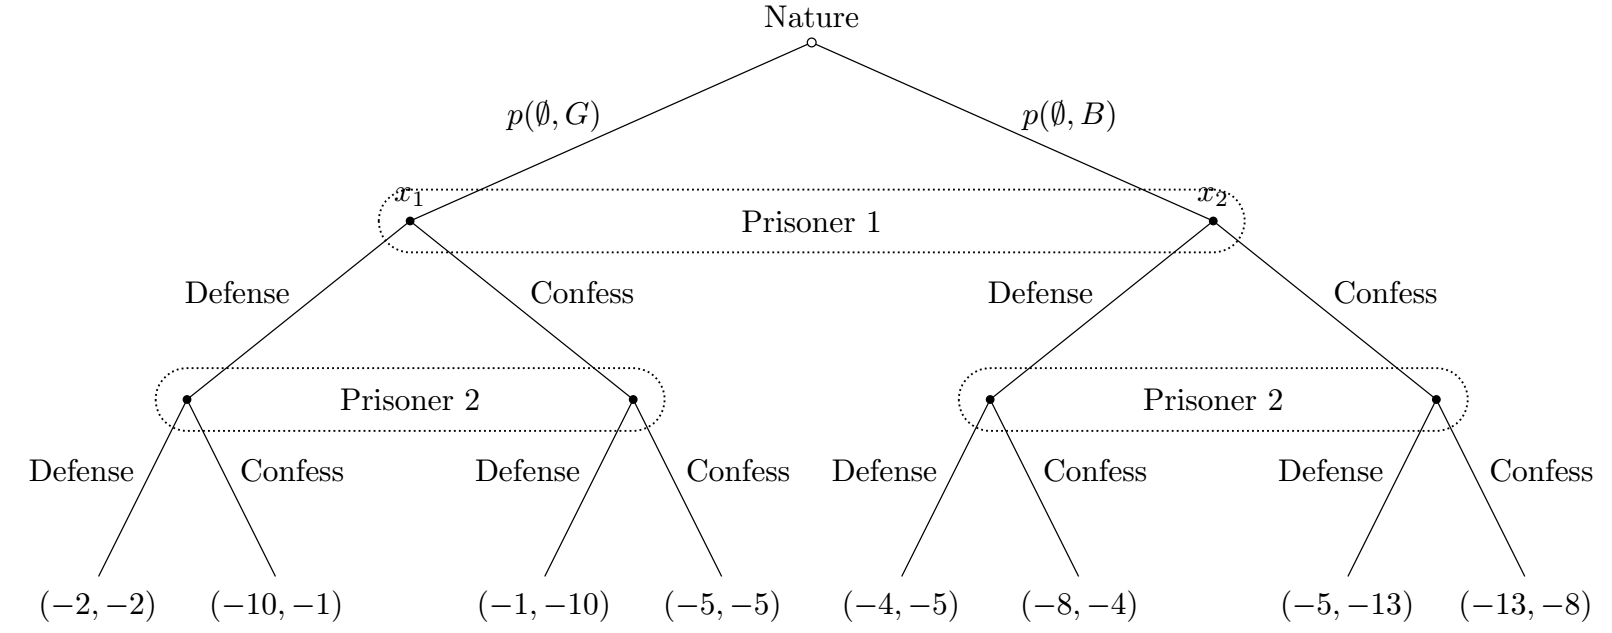
\includegraphics{Figure/incom_tree_bey2.png}
\textit{p} is called the prior belief in the sense that players know this even without knowing their own types. But after observing \( \theta_i \), player \( i \) will update her belief using Bayes rule. She will assign belief to \( (\theta_i, \theta_{-i}) \) conditional on \( \theta_i \). In notation, that is

\[
p(\theta_i, \theta_{-i} | \theta_i) = \frac{p(\theta_i, \theta_{-i})}{\sum_{\theta'_{-i}} p(\theta_i, \theta'_{-i})}
\]

This is called the posterior belief of player \( i \) of type \( \theta_i \).

Now we update the belief of Prisoner 1. This is trivial because Prisoner 1 has only one type.

\[
p(\emptyset, B | \emptyset) = \frac{p(\emptyset, B)}{p(\emptyset, B) + p(\emptyset, G)} = p(\emptyset, B)
\]

This is the probability that Prisoner 1 assigns to \( x_2 \) in her information set.

\[
\mu(x_2) = p(\emptyset, B)
\]

We call \( p(\cdot) \) the prior belief, which is the belief of a player when she has not observed her type yet. We call \( p(\cdot | \theta_i) \) the posterior belief of player \( i \), which is the belief of her after she observed her type.

\subsection{Bayesian Nash Equilibrium}
\subsection{Ex-Ante Optimization}
We know what a strategy is in a Bayesian game. If we define the utility properly, we can directly use the definition of Nash equilibrium here by just changing some notations. Recall the definition of Nash equilibrium.

\textbf{Definition 4.} A strategy profile \( \sigma = (\sigma_1, \sigma_2, \dots, \sigma_n) \) constitutes a Nash equilibrium of 
\[
\Gamma_N = [I, \{\Delta(S_i)\}_{i\in I}, \{u_i(\cdot)\}_{i\in I}]
\]
if for every \( i = 1, \dots, n \),
\[
u_i(\sigma_i, \sigma_{-i}) \geq u_i(\sigma'_i, \sigma_{-i})
\]
for all \( \sigma'_i \in \Delta(S_i) \).

We now extend this to include types. Firstly, the strategy and the payoff should now be relevant to the type profile. Thus, we need to replace \( u_i(\sigma_i, \sigma_{-i}) \) by
\[
u_i(\sigma_i(\theta_i), \sigma_{-i}(\theta_{-i}), \theta_i, \theta_{-i})
\]

*Note: my payoff is related to my strategies, type and others’ types. Other players’ payoffs are similarly defined.

If we use this in the definition, it will become the ex-post equilibrium. And we know that ex-post equilibrium may not exist. Let's now think about the probability of the above type profile, that will be

\[
p(\theta_i, \theta_{-i})
\]

when there are finite or countably infinite types, or

\[
p(\theta_i, \theta_{-i}) d\theta
\]

when there are uncountably infinite types.

With the probability, we can now define the expected payoff of a player \( i \) when players choose strategy profile \( \sigma = (\sigma_1, \sigma_2, \dots, \sigma_n) \).

\[
\sum_{\theta \in \Theta} p(\theta_i, \theta_{-i}) u_i(\sigma_i(\theta_i), \sigma_{-i}(\theta_{-i}), \theta_i, \theta_{-i})
\]

or

\[
\int_{\theta \in \Theta} p(\theta_i, \theta_{-i}) u_i(\sigma_i(\theta_i), \sigma_{-i}(\theta_{-i}), \theta_i, \theta_{-i}) d\theta
\]

Both of them will be denoted as

\[
E[u_i(\sigma_i(\theta_i), \sigma_{-i}(\theta_{-i}), \theta_i, \theta_{-i})]
\]

Then, we have done all our preparations. We can now define the Nash equilibrium in a Bayesian game, which is called the Bayesian Nash equilibrium.

\textbf{Definition 5.} A strategy profile \( \sigma = (\sigma_1, \sigma_2, \dots, \sigma_n) \) constitutes a Bayesian Nash equilibrium of game
\[
\Gamma_N = [I, \{\Delta(A_i)\}_{i\in I}, \{u_i(\cdot)\}_{i\in I}, \{\Theta_i\}_{i\in I}, p(\cdot)]
\]
if for every \( i = 1, \dots, n \),

\[
E[u_i(\sigma_i(\theta_i), \sigma_{-i}(\theta_{-i}), \theta_i, \theta_{-i})] \geq E[u_i(\sigma'_i(\theta_i), \sigma_{-i}(\theta_{-i}), \theta_i, \theta_{-i})]
\]

for all \( \sigma'_i \).

*NOTE: I optimize my strategy given my different type, others' strategies and types. Other players do the same. I don't know my type, but I know the probability of my type. I optimize my strategy given this probability.

This is called ex-ante because in the above definition, a player has not observed her own type. You can imagine that she is choosing what (mixed) action she is going to take when she knows her type. And she makes the plans for each possible type.

From the definition, we can see that a weakly dominant strategy equilibrium is a Bayesian Nash equilibrium. One can see that by multiplying both sides of the following inequality by a probability and then adding over all possible strategy profiles.

\[
u_i(\sigma_i(\theta_i), a_{-i}, \theta_i, \theta_{-i}) \geq u_i(\sigma'_i(\theta_i), a_{-i}, \theta_i, \theta_{-i})
\]

Now come back to the discussion of our example, suppose \( p(\emptyset, G) = \frac{1}{3} \) and \( p(\emptyset, B) = \frac{2}{3} \).

We first find out whether there is a pure-strategy Bayesian Nash equilibrium such that each player of each type always chooses a pure action. P1 has two pure strategies: D and C. P2 has 4 pure strategies: (D,D), (D,C), (C,D), and (D,D). In each tuple, the first element represents his action when his type is G and the second element represents his action when his type is B. Or we can explain them using the game tree.

We can now rewrite the game in the following normal form, where each row represents a pure strategy of P1 and each column represents a pure strategy of P2.

\begin{table}[h]
    \centering
    \renewcommand{\arraystretch}{1.5}
    \setlength{\tabcolsep}{12pt}
    \begin{tabular}{c|c c c c}
        \multicolumn{1}{c}{} & \multicolumn{4}{c}{\textbf{P2}} \\
        \multicolumn{1}{c}{} & (D,D) & (D,C) & (C,D) & (C,C) \\
        \hline
        \textbf{P1} & & & & \\
        D & & & & \\
        C & & & & \\
    \end{tabular}
\end{table}

Now we need to decide the payoffs. Notice that even though we are just considering the pure strategies of players, we have to consider expected payoff because we don’t know what types the nature choose.

As an example, consider the case where P1 chooses D, and P2 chooses (C,D). With probability \( p(\emptyset, G) = \frac{1}{3} \), the outcome will be (D,C), which yields payoffs (-10,-1). With probability \( p(\emptyset, B) = \frac{2}{3} \), the outcome will be (D,D), which yields payoffs (-4,-5). Thus, the expected payoffs should be 

\[
\left( -6, -\frac{11}{3} \right).
\]

Let's do this for all other pure strategy profiles.

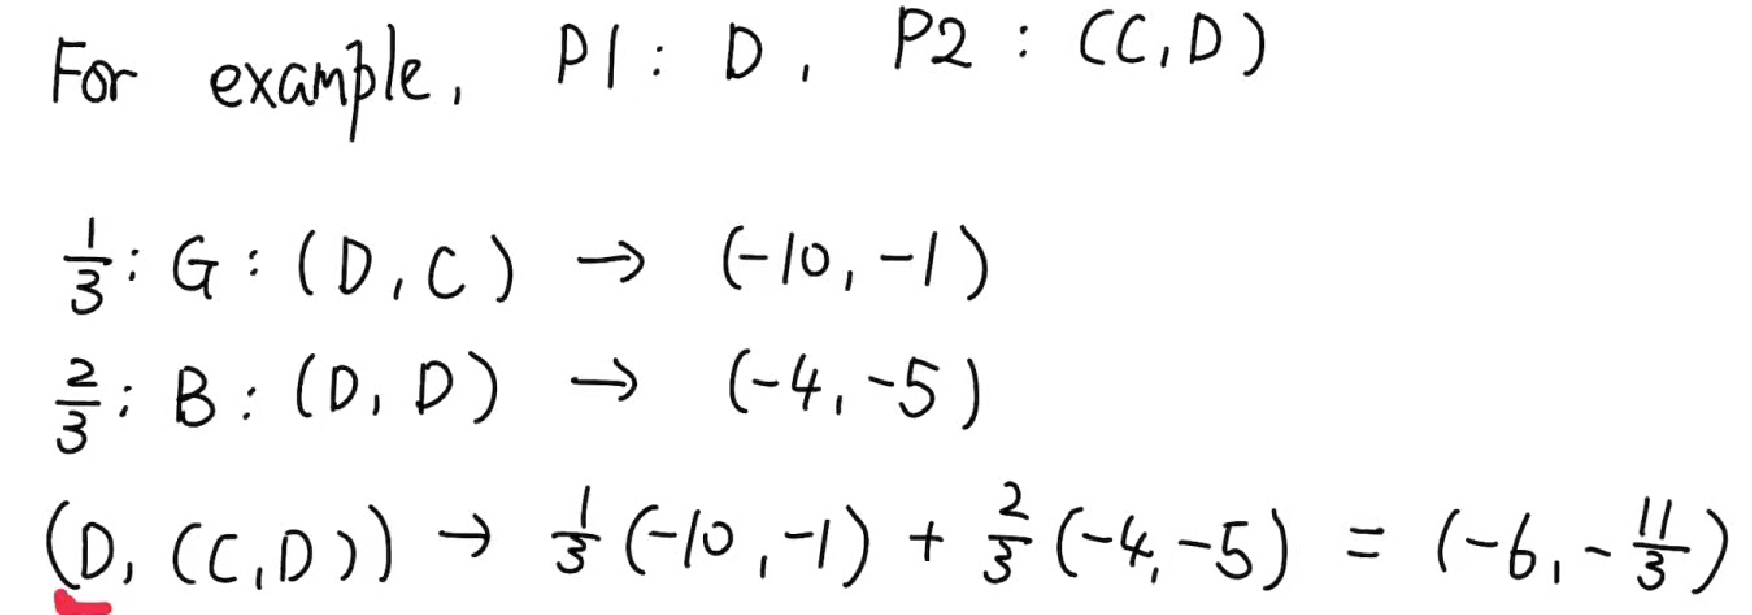
\includegraphics{Figure/cpt_process1.png}



\begin{table}[h]
    \centering
    \renewcommand{\arraystretch}{1.5}
    \setlength{\tabcolsep}{8pt}
    \begin{tabular}{c|c|c|c|c|c|c|c}
        \toprule
        \textbf{P1} & \textbf{P2} & \( (\emptyset, G) \) & \( p(\emptyset, G) \) & \( (\emptyset, B) \) & \( p(\emptyset, B) \) &  & \textbf{Payoffs} \\
        \midrule
        \multirow{4}{*}{D} & (D,D) & (-2,-2) & \( \frac{1}{3} \) & \( \left(-\frac{2}{3}, -\frac{2}{3} \right) \) & (-4,-5) & \( \left(-\frac{8}{3}, -\frac{10}{3} \right) \) & \( \left(-\frac{10}{3}, -4 \right) \) \\
        & (D,C) & (-2,-2) & \( \frac{1}{3} \) & \( \left(-\frac{2}{3}, -\frac{2}{3} \right) \) & (-8,-4) & \( \left(-\frac{16}{3}, -\frac{8}{3} \right) \) & \( (-6,-\frac{10}{3}) \) \\
        & (C,D) & (-10,-1) & \( \frac{1}{3} \) & \( \left(-\frac{10}{3}, -\frac{1}{3} \right) \) & (-4,-5) & \( \left(-\frac{8}{3}, -\frac{10}{3} \right) \) & \( (-6,-\frac{11}{3}) \) \\
        & (C,C) & (-10,-1) & \( \frac{1}{3} \) & \( \left(-\frac{10}{3}, -\frac{1}{3} \right) \) & (-8,-4) & \( \left(-\frac{16}{3}, -\frac{8}{3} \right) \) & \( \left(-\frac{26}{3}, -3 \right) \) \\
        \midrule
        \multirow{4}{*}{C} & (D,D) & (-1,-10) & \( \frac{1}{3} \) & \( \left(-\frac{1}{3}, -\frac{10}{3} \right) \) & (-5,-13) & \( \left(-\frac{10}{3}, -\frac{26}{3} \right) \) & \( \left(-\frac{11}{3}, -12 \right) \) \\
        & (D,C) & (-1,-10) & \( \frac{1}{3} \) & \( \left(-\frac{1}{3}, -\frac{10}{3} \right) \) & (-13,-8) & \( \left(-\frac{26}{3}, -\frac{16}{3} \right) \) & \( (-9,-\frac{26}{3}) \) \\
        & (C,D) & (-5,-5) & \( \frac{1}{3} \) & \( \left(-\frac{5}{3}, -\frac{5}{3} \right) \) & (-5,-13) & \( \left(-\frac{10}{3}, -\frac{26}{3} \right) \) & \( (-5,\frac{31}{3}) \) \\
        & (C,C) & (-5,-5) & \( \frac{1}{3} \) & \( \left(-\frac{5}{3}, -\frac{5}{3} \right) \) & (-13,-8) & \( \left(-\frac{26}{3}, -\frac{16}{3} \right) \) & \( \left(-\frac{31}{3}, -7 \right) \) \\
        \bottomrule
    \end{tabular}
\end{table}

Then we can fill in the table.

\begin{table}[h]
    \centering
    \renewcommand{\arraystretch}{1.5}
    \setlength{\tabcolsep}{12pt}
    \begin{tabular}{c|c|c|c|c}
        \multicolumn{1}{c}{} & \multicolumn{4}{c}{\textbf{P2}} \\
        \multicolumn{1}{c}{} & (D,D) & (D,C) & (C,D) & (C,C) \\
        \hline
        D & \( \left(-\frac{10}{3}, -4 \right) \) & \( (-6, -\frac{10}{3}) \) & \( (-6, -\frac{11}{3}) \) & \( \left(-\frac{26}{3}, -3 \right) \) \\
        C & \( \left(-\frac{11}{3}, -12 \right) \) & \( (-9, -\frac{26}{3}) \) & \( (-5, -\frac{31}{3}) \) & \( \left(-\frac{31}{3}, -7 \right) \) \\
    \end{tabular}
\end{table}

If we successfully find the above matrix, we can now forget about the fact that we are dealing with a
Bayesian game. We can treat the above game as a complete information game and find the equilibrium in the
usual way.

\subsection{Optimization by `Type' Players}
Another equivalent definition of Bayesian Nash equilibrium assumes players observe their types. Then they update their beliefs about others’ types and then choose the optimal action given others’ strategies.

After observing her own type \( \theta_i \), player \( i \)’s expected payoff from the strategy profile \( \sigma = (\sigma_1, \sigma_2, \dots, \sigma_n) \) can be written as

\[
\sum_{\theta_{-i} \in \Theta_{-i}} p(\theta_i, \theta_{-i} | \theta_i) u_i(\sigma_i(\theta_i), \sigma_{-i}(\theta_{-i}), \theta_i, \theta_{-i})
\]

or

\[
\int_{\theta_{-i} \in \Theta_{-i}} p(\theta_i, \theta_{-i} | \theta_i) u_i(\sigma_i(\theta_i), \sigma_{-i}(\theta_{-i}), \theta_i, \theta_{-i}) d\theta_{-i}
\]

Both of them will be denoted as

\[
E[u_i(\sigma_i(\theta_i), \sigma_{-i}(\theta_{-i}), \theta_i, \theta_{-i}) | \theta_i]
\]

Then we can define the Bayesian Nash equilibrium as the following.

\textbf{Definition 6.} A strategy profile \( \sigma = (\sigma_1, \sigma_2, \dots, \sigma_n) \) constitutes a Bayesian Nash equilibrium of game 

\[
\Gamma_N = [I, \{\Delta(A_i)\}_{i\in I}, \{u_i(\cdot)\}_{i\in I}, \{\Theta_i\}_{i\in I}, p(\cdot)]
\]

if for every type \( \theta_i \) of player \( i = 1, \dots, n \),

\[
E[u_i(\sigma_i(\theta_i), \sigma_{-i}(\theta_{-i}), \theta_i, \theta_{-i}) | \theta_i] \geq E[u_i(a'_i, \sigma_{-i}(\theta_{-i}), \theta_i, \theta_{-i}) | \theta_i]
\]

for all \( a'_i \in A_i \).

It is easy to check that this definition is equivalent to the last definition.

The good thing about using this definition is that we can treat each type of a player as a “type” player. The reason is that the action of a type of a player has no influence on the payoff of a different type of the same player.

So, in our example, we can imagine there are 3 players. P1, P2 of type G, and P2 of type B. Then the game can be thought of as a three-player game, with P1 being the row player, P2 of type G being the column player, and P2 of type B being the matrix player.

\subsection{Application}
\subsubsection{Cournot Competition with Incomplete Information}
Consider the Cournot competition with two firms we have talked about. For simplicity, assume that the inverse demand function is given by the following.

\[
p(q_1, q_2) = 2 - (q_1 + q_2)
\]

That is, when the total output is too large, the price could be negative and the firms still have to produce and get a negative profit.

Suppose firm 1’s marginal cost is 1. On the other hand, firm 2’s marginal cost could be either \( \frac{3}{4} \) or \( \frac{5}{4} \), with equal probabilities.

This is a Bayesian game where firm 1 has one type and firm 2 has two types. We treat the two types of firm 2 as different players. The pure strategies of the players can be denoted as \( q_1 \), \( q_2(L) \), and \( q_2(H) \), respectively.

Firm 1 solves the following problem.
\[
\max_{q_1} \frac{1}{2} \left[ (2 - q_1 - q_2(L)) q_1 - q_1 \right] 
+ \frac{1}{2} \left[ (2 - q_1 - q_2(H)) q_1 - q_1 \right]
\] = \[
\max_{q_1} \left( 1 - q_1 - \left( \frac{1}{2} q_2(L) + \frac{1}{2} q_2(H) \right) \right) q_1
\]

Firm 2 with low cost solves the following problem.

\[
\max_{q_2(L)} \left( \frac{5}{4} - q_1 - q_2(L) \right) q_2(L)
\]

Firm 2 with high cost solves the following problem.

\[
\max_{q_2(H)} \left( \frac{3}{4} - q_1 - q_2(H) \right) q_2(H)
\]

We can have the following 3 FOCs:

\[
1 - 2q_1 - \left( \frac{1}{2} q_2(L) + \frac{1}{2} q_2(H) \right) = 0
\]

\[
\frac{5}{4} - q_1 - 2q_2(L) = 0
\]

\[
\frac{3}{4} - q_1 - 2q_2(H) = 0
\]

Solving the above, we have \( q_1 = \frac{1}{3} \), \( q_2(L) = \frac{11}{24} \), and \( q_2(H) = \frac{5}{24} \).

--------------------------------------------------------------------------------------------------------------------
\subsubsection{Bertrand with Incomplete Information}
\textbf{Exercise: Betrend Competition} 

Consider the following asymmetric-information model of Bertrand duopoly with differentiated products. Demand for firm \( i \) is 

\[
q_i(p_i, p_j) = a - p_i - b_i \cdot p_j.
\]

Costs are zero for both firms. The sensitivity of firm \( i \)'s demand to firm \( j \)'s price is either high or low. That is, \( b_i \) is either \( b_H \) or \( b_L \), where \( b_H > b_L > 0 \). For each firm, \( b_i = b_H \) with probability \( \theta \) and \( b_i = b_L \) with probability \( 1 - \theta \), independent of the realization of \( b_j \). 

Each firm knows its own \( b_i \) but not its competitor’s. All of this is common knowledge. Solve for the Bayesian Nash equilibrium.

\textbf{Solution:}
We look for a symmetric pure strategy Bayesian Nash equilibrium:

\[
p^*: \{b_H, b_L\} \to \{p^*_H, p^*_L\}.
\]

So that each firm chooses \( p^*_H \) if \( b_i = b_H \) and \( p^*_L \) if \( b_i = b_L \).

Given that firm 2 follows such BNE, firm 1 with \( b_i \) solves the following maximization problem:

\[
\max_{p_i} \mathbb{E}_{b_j} [p_i (a - p_i - b_i p^*(b_j))]
\]

\[
= p_i [a - p_i - b_i (\theta p^*_H + (1 - \theta) p^*_L)].
\]

\textbf{F.O.C is}

\[
a - p_i - b_i (\theta p^*_H + (1 - \theta) p^*_L) - p_i = 0 \Rightarrow
\]

\[
p^*_i = \frac{1}{2} [a - b_i (\theta p^*_H + (1 - \theta) p^*_L)].
\]

For \( p^* \) to constitute a symmetric BNE, we must have \( p^*_i = p^*_H \) if \( b_i = b_H \) and \( p^*_i = p^*_L \) if \( b_i = b_L \). Hence the F.O.C. implies

\[
p^*_H = \frac{1}{2} [a - b_H (\theta p^*_H + (1 - \theta) p^*_L)]
\]

\[
p^*_L = \frac{1}{2} [a - b_L (\theta p^*_H + (1 - \theta) p^*_L)].
\]

\[
a = (2 + \theta b_H) p^*_H + (1 - \theta) b_H p^*_L
\]

\[
a = \theta b_L p^*_H + (2 + (1 - \theta) b_L) p^*_L
\]

The above two conditions characterize a symmetric pure strategy BNE.

We can easily show that

\[
p^*_H = \frac{[2 - (1 - \theta)(b_H - b_L)]}{[2 + \theta(b_H - b_L)]} p^*_L.
\]

Substitute this into the equilibrium conditions, then get,

\[
p^*_H = \frac{a [2 - (1 - \theta)(b_H - b_L)]}{2 [2 + \theta b_H + (1 - \theta) b_L]}
\]

\[
p^*_L = \frac{a [2 + \theta (b_H - b_L)]}{2 [2 + \theta b_H + (1 - \theta) b_L]}
\]

(which are non-negative if \( 2 - (1 - \theta)(b_H - b_L) \geq 0 \) or equivalently \( b_L + \frac{2}{1-\theta} \geq b_H \)).



\subsubsection{Auction with Incomplete Information}
We will consider an important application of incomplete information static games.  

\textbf{(1) Independent Private Values}

A seller is going to sell a good. There are \( n \) potential buyers. Let \( \theta_i \) be the valuation of buyer \( i \), which is the maximum amount buyer \( i \) is willing to pay for the object. Each buyer knows her own valuation, but not other buyers’ valuations.

Suppose \( \theta_1, \theta_2, \dots, \theta_n \) are independently and identically distributed on interval \( [0, \bar{\theta}] \) according to a distribution function \( F \) with probability density function \( f = F' \). This is a common knowledge among all buyers.

This is called the independent private values (IPV) setting, where each buyer’s value of the good is not related to other buyers’ values. We will focus on this setting.

We will consider two types of auctions through which the seller sells the good. We will call the buyers bidders from now on.

\textbf{(2) Second-Price Sealed-Bid Auction}

In a second-price sealed-bid auction, each bidder writes down his bid and places it in an envelope. Then the envelopes are opened simultaneously. The highest bidder wins the auction and pays a price equal to the second-highest bid or the highest-losing bid. Assume that if there is a tie, no one wins.

Let \( b_i \) denote the bid of bidder \( i \). Then we can write down the payoff of bidder \( i \) as the following.

\[
u_i(b_i, b_{-i}, \theta_i) =
\begin{cases}
\theta_i - \max_{j \neq i} b_j & \text{if } b_i > \max_{j \neq i} b_j \\
0 & \text{if } b_i \leq \max_{j \neq i} b_j
\end{cases}
\]

We don’t include other bidders’ valuations in the payoff of bidder \( i \) because they do not influence bidder \( i \)’s payoff.

A pure strategy of bidder \( i \) is a function \( s_i : [0, \bar{\theta}] \to [0, \infty) \), such that \( s_i(\theta_i) \) is the bid of bidder \( i \) when his valuation is \( \theta_i \).

A weakly dominant strategy of bidder \( i \) is \( s_i(\theta_i) = \theta_i \), i.e., each bidder bids her own valuation. To see this, first consider the payoff of bidder \( i \) when she bids \( b_i > \theta_i \) instead. Let \( b_j \) be the highest bid of other players.

\begin{enumerate}
    \item If \( b_j < b_i \), buyer \( i \) still wins and pays the same amount \( b_j \). Her payoff does not change.
    \item If \( b_i > b_j < \theta_i \), buyer \( i \) loses. Her payoff decreases from \( \theta_i - b_j \) to \( 0 \).
    \item If \( b_j \geq \theta_i \), buyer \( i \) still loses. Her payoff does not change.
\end{enumerate}

Next, consider the payoff of bidder \( i \) when she bids \( b_i > \theta_i \) instead. Let \( b_j \) be the highest bid of other players.

\begin{enumerate}
    \item If \( b_j < \theta_i \), buyer \( i \) still wins and pays the same amount \( b_j \). Her payoff does not change.
    \item If \( \theta_i \leq b_j < b_i \), buyer \( i \) wins. Her payoff decreases from \( 0 \) to \( \theta_i - b_j \).
    \item If \( b_j \geq b_i \), buyer \( i \) still loses. Her payoff does not change.
\end{enumerate}

Then, we can conclude that there is a weakly dominant strategy equilibrium in the second-price sealed-bid auction, where each bidder bids her own valuation.

\textbf{(3) First Price Sealed-Bid Auction}

In a second-price sealed-bid auction, each bidder writes down his bid and places it in an envelope. Then the envelopes are opened simultaneously. The highest bidder wins the auction and pays her bid. Assume that if there is a tie, no one wins.

Let \( b_i \) denote the bid of bidder \( i \). Then we can write down the payoff of bidder \( i \) as the following:

\[
u_i(b_i, b_{-i}, \theta_i) =
\begin{cases}
\theta_i - b_i & \text{if } b_i > \max_{j \neq i} b_j \\
0 & \text{if } b_i \leq \max_{j \neq i} b_j
\end{cases}
\]

Let’s find a Nash equilibrium of this Bayesian game. We focus on the strategy profile \( (s_1, s_2, \dots, s_n) \) such that \( s_1 = s_2 = \dots = s_n \) and \( s_i(\cdot) \) is a strictly increasing function with \( s_i(0) = 0 \) for all \( i \).

$s_i(\cdot)$ is an increasing function because $s_i$ is increasing with $\theta_i$

This is to say that we focus on symmetric and increasing pure strategies of bidders.

Without loss, consider bidder 1 of type \( \theta_i \). If she bids \( b_1 \), her expected payoff is:

\[
Pr(b_1 > s_2(\theta_2)) \times Pr(b_1 > s_3(\theta_3)) \times \cdots \times Pr(b_1 > s_n(\theta_n)) \times (\theta_1 - b_1)
\]

Here, \( Pr(b_1 > s_i(\theta_i)) \) is the probability that \( b_1 \) is higher than what bidder \( i \) bids. Since bidders’ valuations are independent, the probability that \( b_1 \) wins is 

\[
Pr(b_1 > s_2(\theta_2)) \times Pr(b_1 > s_3(\theta_3)) \times \cdots \times Pr(b_1 > s_n(\theta_n)).
\]

Now we use the assumption that \( s_2 = \dots = s_n \) and \( s_i(\cdot) \) is strictly increasing. Let’s say \( \beta = s_2 = \dots = s_n \). Then there exists \( z \) such that \( \beta(z) = b_i \). Rewrite the expected payoff:

\[
Pr(\beta(z) > \beta(\theta_2)) \times Pr(\beta(z) > \beta(\theta_3)) \times \cdots \times Pr(\beta(z) > \beta(\theta_n)) \times (\theta_1 - \beta(z))
\]

\[
= Pr(z > \theta_2) \times Pr(z > \theta_3) \times \cdots \times Pr(z > \theta_n) \times (\theta_1 - \beta(z))
\]

\[
= [F(z)]^{n-1} \times (\theta_1 - \beta(z))
\]

The first equality uses the assumption that \( \beta \) is strictly increasing. The second equality is the result of identical distribution.

Notice that bidding \( b_1 \) is equivalent to choosing \( z \) now. Because from \( b_1 \), we can use \( \beta \) to uniquely pin down \( z \). Now take the first order condition of the above with respect to \( z \):

\[
(n - 1)[F(z)]^{n-2} f(z) \times (\theta_1 - \beta(z)) - [F(z)]^{n-1} \beta'(z) = 0
\]

What value of \( z \) satisfies the above FOC ? Since we are considering an equilibrium strategy, bidding \( \beta(\theta_1) \) should be optimal. Therefore, \( z = \theta_1 \) satisfies the above FOC.

\[
(n - 1)[F(\theta_1)]^{n-2} f(\theta_1) \times (\theta_1 - \beta(\theta_1)) - [F(\theta_1)]^{n-1} \beta'(\theta_1) = 0
\]

\[
(n - 1)[F(\theta_1)]^{n-2} f(\theta_1) \beta(\theta_1) + [F(\theta_1)]^{n-1} \beta'(\theta_1) = (n - 1)[F(\theta_1)]^{n-2} f(\theta_1) \theta_1
\]

\[
\frac{d}{d\theta_1} ([F(\theta_1)]^{n-1} \beta(\theta_1)) = (n - 1)[F(\theta_1)]^{n-2} f(\theta_1) \theta_1
\]

Let's first replace \( \theta_1 \) by \( t \).

\[
\frac{d}{dt} ([F(t)]^{n-1} \beta(t)) = (n - 1)[F(t)]^{n-2} f(t) t
\]

\[
d ([F(t)]^{n-1} \beta(t)) = (n - 1)[F(t)]^{n-2} f(t) t dt
\]

Then integrate \( t \) from \( 0 \) to \( \theta_1 \), and we have

\[
[F(\theta_1)]^{n-1} \beta(\theta_1) - [F(0)]^{n-1} \beta(0) = \int_0^{\theta_1} (n - 1)[F(t)]^{n-2} f(t) t dt
\]

Here, \( \beta(0) = 0 \) by our assumption. So we have

\[
\beta(\theta_1) = \frac{1}{[F(\theta_1)]^{n-1}} \int_0^{\theta_1} (n - 1)[F(t)]^{n-2} f(t) t dt
\]

Let's deal with the integral a little bit.

\[
\int_0^{\theta_1} (n - 1)[F(t)]^{n-2} f(t) t dt = \int_0^{\theta_1} t d[F(t)]^{n-1}
\]

\[
= \left\{ [F(t)]^{n-1} t \right\} \bigg|_{t=0}^{\theta_1} - \int_0^{\theta_1} [F(t)]^{n-1} dt
\]

\[
= [F(\theta_1)]^{n-1} \theta_1 - \int_0^{\theta_1} [F(t)]^{n-1} dt
\]

Therefore, we have

\[
\beta(\theta_1) = \theta_1 - \int_0^{\theta_1} \frac{[F(t)]^{n-1}}{[F(\theta_1)]^{n-1}} dt
\]

Recall that we consider bidder 1 without loss. Therefore, we have found a Bayesian Nash equilibrium where bidder \( i \) uses a strategy \( s_i \) such that for any \( \theta_i \),

\[
s_i(\theta_i) = \beta(\theta_i) = \theta_i - \int_0^{\theta_i} \frac{[F(t)]^{n-1}}{[F(\theta_i)]^{n-1}} dt
\]

This is lower than \( \theta_i \). That makes sense because otherwise, the bidder's payoff will be 0 or negative.

\textbf{Exercise: first-price sealed-bid auction}

\noindent
\textbf{1.} Consider the first-price sealed bid auction (introduced in the lecture) with two bidders, \( i = 1,2 \).
Each bidder’s valuation is drawn independently from the cumulative distribution \( F(v) \) on \( [0,1] \).

\noindent
\textbf{(a)} Formulate bidder 1’s maximization problem given that bidder 2 follows the equilibrium bid function, \( \sigma(\cdot) \):

\noindent
\textbf{Solution:} We assume that this equilibrium bid function is strictly increasing. Given that bidder 2 follows the equilibrium \( \sigma(\cdot) \), bidder 1’s problem is given by

\[
\max_b (v - b) Pr(b > \sigma(v_2)) = (v - b) F(\sigma^{-1}(b))
\]

\(\blacksquare\)

\noindent
\textbf{(b)} Derive the conditions that characterize the symmetric equilibrium (in which both bidders follow the same strategy \( \sigma \)):

\noindent
\textbf{Solution:} We look for a symmetric equilibrium in which \( \sigma_1 = \sigma_2 = \sigma \). The first-order condition with respect to \( b \):

\[
- F(\sigma^{-1}(b)) + (v - b) f(\sigma^{-1}(b)) \frac{1}{\sigma'(\sigma^{-1}(b))} \Bigg|_{b = \sigma(v)} = 0
\]

\[
- F(v) + (v - \sigma(v)) f(v) \frac{1}{\sigma'(v)} = 0
\]

It is also easily seen that in equilibrium, \( \sigma(0) = 0 \). So the ODE system is given by

\[
(1) \quad -F(v) + (v - \sigma(v)) f(v) \frac{1}{\sigma'(v)} = 0
\]

\[
(2) \quad \sigma(0) = 0
\]

The above two conditions characterize the symmetric pure strategy Bayesian Nash Equilibrium (BNE).

\(\blacksquare\)

\noindent
\textbf{(c)} Solve for the symmetric equilibrium bid function \( \sigma(v) \). 

\noindent
\textbf{Solution:} \textit{[Remark: if you don’t know how to solve an ODE system derived in (c) above to get the solution, you may use the envelope theorem introduced in the lecture.]}

\textbf{• Method \#1 (ODE)}

From equation (1),

\[
- F(v) + (v - \sigma(v)) f(v) \frac{1}{\sigma'(v)} = 0
\]

\[
\Leftrightarrow f(v) \sigma(v) + F(v) \sigma'(v) = v f(v)
\]

\[
\Leftrightarrow \frac{d}{dv} (F(v) \sigma(v)) = \frac{d}{dv} \left(\int_0^v \bar{v} f(\bar{v}) d\bar{v} + C \right)
\]

\[
\Leftrightarrow F(v) \sigma(v) = \int_0^v \bar{v} f(\bar{v}) d\bar{v} + C = \bar{v} F(\bar{v}) \Big|_0^v - \int_0^v F(\bar{v}) d\bar{v} + C
\]

The last equality is followed by the integration by parts.

\[
\Leftrightarrow F(v) \sigma(v) = v F(v) - \int_0^v F(\bar{v}) d\bar{v} + C
\]

From equation (2), \( \sigma(0) = 0 \), implying that \( C = 0 \). Thus,

\[
\sigma(v) = v - \int_0^v \frac{F(\bar{v})}{F(v)} d\bar{v}.
\]

\textbf{• Method \#2 (Envelope Theorem)}

In equilibrium, the expected payoff for a bidder with valuation \( v \) is \( \Pi(v) = \pi(v, \sigma(v)) \).

Notice that

\[
\frac{d \Pi(v)}{dv} = \frac{\partial \pi(v, \sigma(v))}{\partial v} + \frac{\partial \pi(v, \sigma(v))}{\partial \sigma} \times \frac{\partial \sigma(v)}{\partial v}.
\]

By the Envelope Theorem, \( \frac{\partial \pi(v, \sigma(v))}{\partial \sigma} = 0 \).

Consequently,

\[
\frac{d \Pi(v)}{dv} = F(\sigma^{-1}(\sigma(v))) = F(v).
\]

Moreover, notice that

\[
\Pi(v) = (v - \sigma(v)) F(\sigma^{-1}(\sigma(v)))
\]

\[
= (v - \sigma(v)) F(v).
\]

Taking the previous two expressions and substituting them into the identity

\[
\int_0^v \frac{d \Pi(w)}{dw} dw = \Pi(v) - \Pi(0),
\]

we obtain

\[
\int_0^v F(w) dw = (v - \sigma(v)) F(v) - 0.
\]

Rearranging provides an explicit solution \( \sigma(v) \):

\[
\sigma(v) = v - \int_0^v \frac{F(w)}{F(v)} dw,
\]

which is the same as derived in Method \#1.

\(\blacksquare\)

\end{document}
